% Reusable circuit symbols for the tables in Section 2.4.
% All wires run from left to right; for multi-qubit gates the upper wire
% is the leftmost tensor factor.
\tikzset{
  gatetablewire/.style={line width=0.7pt},
  gatetablebox/.style={draw,fill=white,line width=0.7pt,
    minimum width=0.62cm,minimum height=0.56cm,inner sep=1pt}
}

\newcommand{\GateTableSingle}[1]{%
  \begin{tikzpicture}[baseline=(current bounding box.center)]
    \draw[gatetablewire] (0,0) -- (2.4,0);
    \node[gatetablebox] at (1.2,0) {$#1$};
  \end{tikzpicture}%
}

\newcommand{\GateTableControlled}[1]{%
  \begin{tikzpicture}[baseline=(current bounding box.center)]
    \path[use as bounding box] (0,-0.90) rectangle (2.4,0.90);
    \draw[gatetablewire] (0,0.42) -- (2.4,0.42);
    \draw[gatetablewire] (0,-0.42) -- (2.4,-0.42);
    \draw[gatetablewire] (1.2,-0.42) -- (1.2,0.42);
    \fill (1.2,0.42) circle (1.8pt);
    \node[gatetablebox] at (1.2,-0.42) {$#1$};
  \end{tikzpicture}%
}

\newcommand{\GateTableCNOT}{%
  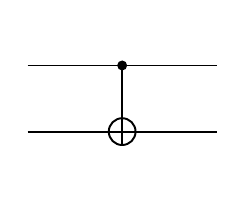
\begin{tikzpicture}[baseline=(current bounding box.center)]
    \path[use as bounding box] (0,-0.90) rectangle (2.4,0.90);
    \draw[gatetablewire] (0,0.42) -- (2.4,0.42);
    \draw[gatetablewire] (0,-0.42) -- (2.4,-0.42);
    \draw[gatetablewire] (1.2,-0.42) -- (1.2,0.42);
    \fill (1.2,0.42) circle (1.8pt);
    \draw[gatetablewire,fill=white] (1.2,-0.42) circle (0.17);
    \draw[gatetablewire] (1.04,-0.42) -- (1.36,-0.42);
    \draw[gatetablewire] (1.2,-0.58) -- (1.2,-0.26);
  \end{tikzpicture}%
}

\newcommand{\GateTableSWAP}{%
  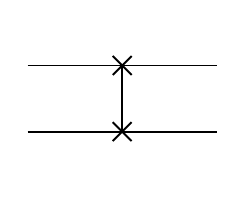
\begin{tikzpicture}[baseline=(current bounding box.center)]
    \path[use as bounding box] (0,-0.90) rectangle (2.4,0.90);
    \draw[gatetablewire] (0,0.42) -- (2.4,0.42);
    \draw[gatetablewire] (0,-0.42) -- (2.4,-0.42);
    \draw[gatetablewire] (1.2,-0.42) -- (1.2,0.42);
    \foreach \y in {0.42,-0.42} {
      \draw[gatetablewire] (1.08,\y-0.12) -- (1.32,\y+0.12);
      \draw[gatetablewire] (1.08,\y+0.12) -- (1.32,\y-0.12);
    }
  \end{tikzpicture}%
}

\newcommand{\GateTableToffoli}{%
  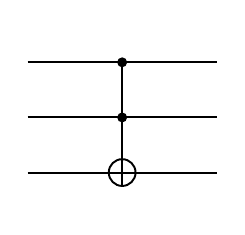
\begin{tikzpicture}[baseline=(current bounding box.center)]
    \path[use as bounding box] (0,-1.14) rectangle (2.4,1.14);
    \foreach \y in {0.70,0,-0.70} {
      \draw[gatetablewire] (0,\y) -- (2.4,\y);
    }
    \draw[gatetablewire] (1.2,-0.70) -- (1.2,0.70);
    \fill (1.2,0.70) circle (1.8pt);
    \fill (1.2,0) circle (1.8pt);
    \draw[gatetablewire,fill=white] (1.2,-0.70) circle (0.17);
    \draw[gatetablewire] (1.04,-0.70) -- (1.36,-0.70);
    \draw[gatetablewire] (1.2,-0.86) -- (1.2,-0.54);
  \end{tikzpicture}%
}
